%!TEX root = thesis.tex

\chapter{Related Work}

	We will now take an in-depth look at some of the results leading up to and related to our own. For definitions of any unfamiliar notation, the reader should refer either to the Preliminaries chapter, or to the cited work that is being discussed. In general, an election will consist of a SCF $f$, a set of $m$ alternatives $C$, $n$ voters, and a profile $p \in L(C)^n$.


\section{Elections Can be Manipulated Often}

	Complexity theorists have analyzed many voting systems using computational complexity as a means of inhibiting manipulation \cite{bartholdi1989computational, hemaspaandra2009hybrid}. Friedgut, Kalai, and Nisan, on the other hand, took a probabilistic approach to this problem \cite{friedgut2008elections}. Instead of studying worst-case manipulation, they performed a probabilistic analysis of random manipulation. That is, instead of a voter intelligently manipulating an election, which can be difficult in terms of worst-case complexity, he simply chooses his manipulation randomly (if his most preferred candidate is not winning already). They proved that even a random manipulation will succeed with non-negligible probability. This is significant because no matter how hard it is in the worst-case to find a profitable manipulation, if it is trivial to find a random manipulation, that could be enough.

	More formally, they defined a metric, \emph{manipulation power} $M_i(f)$, of voter $i$ on a social choice function $f$ to be the probability that $p_i'$ is a profitable manipulation by voter $i$, where $p$ is a profile and $p_i'$ is a preference list which are both chosen uniformly at random. Their main result is that there exists a constant $C$ such that for 3 alternatives, $n$ voters, and a neutral social choice function $f$ that is $\epsilon$-far from dictatorship ($\epsilon > 0$) then

	\begin{align*}
		\sum_{i=1}^n M_i(f) \ge C \epsilon^2.
	\end{align*}

	This means that when $\epsilon$ is fixed---it is fixed once a voting rule is determined---then some voter has more than his share (a non-negligible amount) of manipulation power: $\max_i M_i(f) \ge \Omega(\frac{1}{n})$ \cite{friedgut2008elections}.

	Besides the limitation to three alternatives, these results are incredibly general. They rest on two main assumptions which all common social choice functions satisfy. The first is the \emph{impartial culture assumption} which states that voters are independent and equally likely to select any of the possible orderings of alternatives. In other words, votes are selected uniformly at random. The second assumption is the neutrality of the social choice function. The neutrality assumption was removed by Friedgut, Kalai, and Nisan in 2011 \cite{friedgut2011quantitative}.

	But the restriction to three alternatives renders these results useless for many practical applications, and it is also less satisfactory than a general solution from a theoretical standpoint. Therefore many people have worked to generalize these results.


\section{A sufficient condition for voting rules to be frequently manipulable}

	In 2008 Xia and Conitzer were able to prove a similar theorem for any number of candidates, but instead of neutrality they assumed five other conditions for the voting rule \cite{xia2008sufficient}:

	\begin{description}
		\item[Homogeneity] For any $n \in \mathbb{N}$ we have:
			\begin{align*}
				f(P) = f\left(\bigcup_{i=1}^n P\right).
			\end{align*}
		\item[Anonymity] The result of the election does not depend on the names of the voters. Formally, given a profile $P$ and a permutation $\sigma(P)$ then: $f(P) = f(\sigma(P))$.
		\item[Non-imposition] Every alternative has the possibility of winning.
		\item[Canceling out] Adding the set of all linear orders to the votes does not change the result. More formally, for any profile $P$ we have that: $f(P) = f(P \cup L(C))$.
		\item[Stability] Given alternatives $C = \{c_1, c_2, \ldots, c_m\}$, there exists a profile $P$ such that:
			\begin{enumerate}
				\item $P$ and $D_{m}(P)$ are both stable, i.e. slight modifications don't change the winner. (See below for a definition of $D_{m}$.)
				\item $f(P) = c_1$
				\item $f(D_{m}(P)) = c_2$
			\end{enumerate}
			Where $D_m$ is defined such that if $D_m(P) = P'$, then $P|_{C \backslash \{c_m\}} = P'|_{C \backslash \{c_m\}}$ and the position of $c_m$ is uniformly distributed in $P'$. For a formal definition of $D_m$ and of ``stability,'' see the original paper \cite{xia2008sufficient}.
	\end{description}

	However, these conditions are stricter than the neutrality assumption of Friedgut, Kalai, and Nisan, in the sense that they do not capture all of the ``common'' voting rules, e.g. Bucklin.


\section{Frequent manipulability of elections: The case of two voters}

	Around the same time Dobzinski and Procaccia published complementary results for two voters and social choice functions satisfying unanimity (the Pareto principle) \cite{dobzinski2008frequent}. They proved the following:

	\begin{theorem}[Dobzinski and Procaccia]
		Let $f$ be a Pareto-optimal SCF and let $n = 2$, $m \ge 3$, and $\delta < \frac{1}{32m^9}$. If $f$ is $\delta$-strategyproof then $f$ is $16m^8 \delta$-dictatorial.
	\end{theorem}

	We will translate these results into the same terms used by Friedgut, Kalai, and Nisan so that we can easily compare their results. According to Dobzinski and Procaccia, being $\delta$-strategyproof means that $f$ is manipulable with probability at most $\delta$. This means that if

	\begin{align*}
		\sum_{i=1}^n M_i(f) \le \delta
	\end{align*}

	then $f$ is $16m^8 \delta$-near to dictatorship. If we let $\epsilon = 16m^8 \delta$ then we get that
	\[
		\sum_{i=1}^n M_i(f) \le \frac{\epsilon}{16m^8}
	\]
	implies $f$ is $\epsilon$-near to dictatorship. Or that
	\[
		\sum_{i=1}^n M_i(f) \ge \frac{\epsilon}{16m^8}
	\]
	implies $f$ is $\epsilon$-far from dictatorship. And since $\delta < \frac{1}{32m^9}$, we have $\epsilon < \frac{1}{2m}$. So we can reword their theorem as follows.

	\begin{theorem}[Dobzinski and Procaccia reworded]
		Let $f$ be a Pareto-optimal SCF and let $n = 2$, $m \ge 3$, and $\epsilon < \frac{1}{2m}$. If $\sum_{i=1}^n M_i(f) \ge \frac{\epsilon}{16m^8}$ then $f$ is $\epsilon$-far from dictatorship.
	\end{theorem}

	The limitation of these results to two voters makes them unsuitable for application to political elections because any political election with only two voters seems meaningless. However, Dobzinski and Procaccia point out that even without extending these results there are some social choice situations which have only two voters but many alternatives---and these results are more interesting as the number of alternatives becomes very large. One example of this would be a couple deciding where to eat dinner. There are only two ``voters,'' but there can be a huge number of alternatives to choose from. This kind of situation can also occur among artificial intelligence agents deciding among a vast number of alternatives.


\section{The geometry of manipulation: A quantitative proof of the Gibbard-Satterthwaite theorem}

	In 2010 Isaksson, Kindler, and Mossel published a brilliant generalization of the original theorem of Friedgut, Kalai, and Nisan and even improved slightly upon the results \cite{isaksson2010geometry}. Translating their results into the terminology we have been using, they proved that for a neutral social choice function $f$ with $m \ge 4$ alternatives and $n$ voters that is $\epsilon$-far from dictatorship, a uniformly chosen profile will be manipulable with probability at least $2^{-1} \epsilon^2 n^{-4} m^{-6} (m!)^{-3}$. In other words

	\begin{align*}
		\sum_{i=1}^n M_i(f) \ge \frac{\epsilon^2}{2 n^4 m^6 (m!)^3}.
	\end{align*}

	This bound allows the manipulating voter to randomly permute his entire preference list, which is the case considered by Friedgut, Kalai, and Nisan. However if we restrict him to permuting only four adjacent alternatives, Isaksson, Kindler, and Mossel showed that the bound becomes polynomial in the number of alternatives:

	\begin{align*}
		\sum_{i=1}^n M_i(f) \ge \frac{\epsilon^2}{10^4 n^3 m^{30}}.
	\end{align*}

	Isaksson, Kindler, and Mossel used purely geometric and combinatorial methods to achieve their results. One of the foundational techniques they employed was the canonical path method \cite{jerrum1993polynomial}. Given a graph $G$, the canonical path method attempts to give a lower bound on the `surface area' of a subset of vertices, $A$. Surface area is defined as the number of vertices in $A$ which have an edge to at least one vertex outside of $A$. Given two vertices $x, y$ such that $x \in A$ and $y \notin A$, we call the path between them the canonical path, and clearly this path must contain at least one surface vertex. Then by proving that each surface vertex lies on at most $r$ canonical paths, we bound the surface area of $A$ below by $\frac{|A| |\overline{A}|}{r}$ because the total number of total canonical paths is $|A| |\overline{A}|$.

	The graph used by Isaksson, Kindler, and Mossel is very similar to the one used by Friedgut, Kalai, and Nisan. It is also similar to the one used for the results in this thesis, except that ours is directed, and is missing certain edges.

	Next we define the boundary of $f$ with respect to alternatives $a, b$ as
	\[
		B^{a,b}_i(f) = \{(x, x') \mid f(x) = a, f(x') = b, \forall j \neq i: x_j = x'_j\}.
	\]
	For any distinct alternatives $a, b, c, d$ we construct canonical paths between $B^{a,b}_i$ and $B^{c,d}_j$ such that each path passes through a manipulation point. These paths are called manipulation paths.

	We define manipulation paths between pairs of profiles in $B^{a,b}_i$ and $B^{c,d}_j$. In the first half of the path we will preserve the order or $a, b$, while in the second half of the path we will only modify the order of $a, b$ and not any other alternatives. The length of the manipulation path will be $2n - 3$ because we are not modifying the last two indices. For any pair of profiles $(x, x') \in B^{a,b}_i$ and $(z, z') \in B^{c,d}_j$ we formally define the manipulation path as follows. The manipulation path is of the form:
	\begin{align*}
		(x^{(0)}, x^{\prime(0)}), \ldots, (x^{(n - 2)}, x^{\prime(n - 2)}), (z^{(n - 2)}, z^{\prime(n - 2)}), \ldots, (z^{(0)}, z^{\prime(0)})
	\end{align*}
	such that $(x^{(0)}, x^{\prime(0)}) = (x, x')$ and $(z^{(0)}, z^{\prime(0)}) = (z, z')$. For all $k \in \{0, \ldots, n - 2\}$, and all $s \in \{0, \ldots, n - 2\}$ such that $s \neq k$ we restrict the path so that:
	\begin{align}
		(x_s^{(k)}, x_s^{\prime(k)}) &= (x_s^{(k-1)}, x_s^{\prime(k-1)}) \label{eq:manipulation-path-rule-1-x} \\
		(z_s^{(k)}, z_s^{\prime(k)}) &= (z_s^{(k-1)}, z_s^{\prime(k-1)}). \label{eq:manipulation-path-rule-1-z}
	\end{align}
	Now at the $k$\textsuperscript{th} step we update the $k$\textsuperscript{th} index to have the same ordering of $a, b$ as $(x_k^{(0)}, x_k^{\prime(0)})$ and the same ordering of all other alternatives as $(z_k^{(0)}, z_k^{\prime(0)})$:
	\begin{align}
		(x_k^{(0)}, x_k^{\prime(0)}) &=_{\{a, b\}} (x_k^{(k)}, x_k^{\prime(k)}) =_{\overline{\{a, b\}}} (z_k^{(0)}, z_k^{\prime(0)}) \label{eq:manipulation-path-rule-2-x} \\
		(x_k^{(0)}, x_k^{\prime(0)}) &=_{\{a, b\}} (z_k^{(k)}, z_k^{\prime(k)}) =_{\overline{\{a, b\}}} (z_k^{(0)}, z_k^{\prime(0)}). \label{eq:manipulation-path-rule-2-z}
	\end{align}
	Note that by the pairwise notation for defining a path: $(x^{(0)}, x^{\prime(0)}), (x^{(1)}, x^{\prime(1)})$, we mean that we have two paths of equal length: $x^{(0)}, x^{(1)}$ and $x^{\prime(0)}, x^{\prime(1)}$. Additionally, by the notation $x_k =_D z_k$ we mean that the preference lists $x_k$ and $z_k$ have the same ordering for every alternative in the set $D$ (see Definition \ref{preference-restriction-definition}).

	We will perform a small example to illustrate how the above rules work together in forming the manipulation path. We use $n = 4$ voters which means we will have a manipulation path of length $2n - 3 = 5$. Here, for simplicity, we show only $x$ and $z$ but the example for $x'$ and $z'$ is exactly the same.
	\begin{center}
		\begin{tabular}{r | c c c c c c}
			step						&	0		&	1		&	2		&	2		&	1		&	0		\\
			\hline
			1\textsuperscript{st} index	&	$x_1$	&	$y_1$	&	$y_1$	&	$y_1$	&	$y_1$	&	$z_1$	\\
			2\textsuperscript{nd} index	&	$x_2$	&	$x_2$	&	$y_2$	&	$y_2$	&	$z_2$	&	$z_2$	\\
			3\textsuperscript{rd} index	&	$x_3$	&	$x_3$	&	$x_3$	&	$z_3$	&	$z_3$	&	$z_3$	\\
			4\textsuperscript{th} index	&	$x_4$	&	$x_4$	&	$x_4$	&	$z_4$	&	$z_4$	&	$z_4$	\\
		\end{tabular}
	\end{center}
	Here $y_i$ for $i \in \{1, 2, 3, 4\}$ represents the result of Equation \ref{eq:manipulation-path-rule-2-x} (or \ref{eq:manipulation-path-rule-2-z} depending on whether it's on the $x$ side or the $z$ side). Therefore $y_i$ can be defined as
	\[
		x_i =_{\{a, b\}} y_i =_{\overline{\{a, b\}}} z_i
	\]
	or in other words we get $y_i$ by taking $z_i$ and swapping $a, b$ if necessary to ensure that their order is the same as in $x_i$.

	Another example of a manipulation path is illustrated in Figure \ref{fig:manipulation-path}. In order to keep the figure simple we use $n = 3$ and $m = 4$ and only show one dimension (the ``front'') of the graph, when in reality it would be 3-dimensional. Notice that the $(n - 1)^{th}$ and $n^{th}$ (in this case 2\textsuperscript{nd} and 3\textsuperscript{rd}) indices of the nodes differ. In this highly simplified example the 1\textsuperscript{st} index of $x$, $x^{(1)}$, and $z$ are all the same. Usually they would be different, but still following the constraint
	\[
		x =_{\{a, b\}} x^{(1)} =_{\overline{\{a, b\}}} z.
	\]
	\begin{figure}[ht]
		\begin{center}
			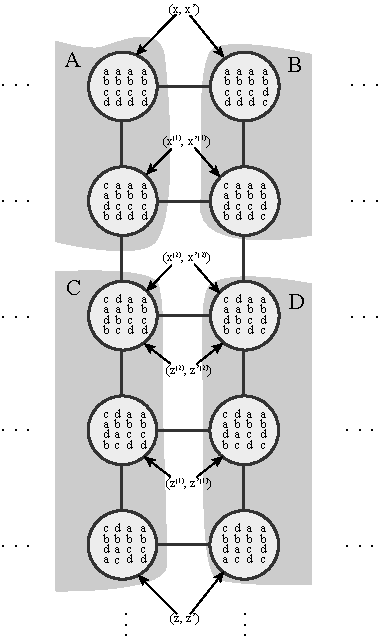
\includegraphics[width=5in]{../figures/diagram7.pdf}
			\caption{A visual example of a manipulation path.}
			\label{fig:manipulation-path}
		\end{center}
	\end{figure}


	We will now go through the example table step by step for the $x$ side (left half); the $z$ side is simply a mirror image of what happens in the $x$ side. At step 0 we have $x^{(0)} = x$ because we specified above that our initial value was $(x^{(0)}, x^{\prime(0)}) = (x,x')$. At step 1 we first use Equation \ref{eq:manipulation-path-rule-1-x} to essentially copy over every index from step 0 except index 1 (because it is the $k$\textsuperscript{th} index during this step). We then apply Equation \ref{eq:manipulation-path-rule-2-x} to index 1 to get $y_1$. At step 2 we again use Equation \ref{eq:manipulation-path-rule-1-x} to copy over every index from step 1 except for index 2 for which we use Equation \ref{eq:manipulation-path-rule-2-x} to get $y_2$. We don't modify the last two indices because these are the only ones on which $x, x'$ and $z, z'$ differ: recall that $(x, x') \in B_{n-1}^{a,b}$ and $(z, z') \in B_{n}^{c,d}$.

	\begin{lemma}[Lemma 5.1 of Isaksson, Kindler, and Mossel]
		For any SCF $f$, distinct $i, j \in \{1, \ldots, n\}$ and distinct alternatives $a, b, c, d \in C$ there exists a mapping $h : B_i^{a,b}(f) \times B_j^{c,d}(f) \rightarrow M$ where
		\[
			M = \{x \in P \mid f \text{ is manipulable at x}\}
		\]
		such that for any $x \in M$
		\[
			|h^{-1}(x)| \le 2n(m!)^{n+4}
		\]
	\end{lemma}
	\begin{proof}
		Without loss of generality, let $i = n - 1$ and $j = n$. We construct a manipulation path between $(x, x') \in B_i^{a,b}(f)$ and $(z, z') \in B_j^{c,d}(f)$. Notice that $(x, x')$ takes the values $(a, b)$ while $(z, z')$ takes the values $(c, d)$ because $f(x) = a$, $f(x') = b$, $f(z) = c$, and $f(z') = d$. Our claim is that along this manipulation path is an edge $((u, u'), (v, v'))$ such that either
		\begin{enumerate}
			\item at least one of $u, u', v, v'$ is a manipulation point
			\item $f$ takes on at least three values on the points $u, u', v, v'$.
		\end{enumerate}
		In explanation, notice that there are at most three possible situations, and at least one of the above claims holds for each:
		\begin{itemize}
			\item On the first half of the path the value of the pair changes from $(a, b)$ to something else. If the first value changes to $b$ or the second value changes to $a$ then we have a manipulation point because the ranking of $a, b$ doesn't change on the first half of the path. Otherwise the values change to something other than $a$ or $b$, so $f$ takes at least three values at this point.
			\item On the second half of the path the value of the pair changes from $(c, d)$ to something else --- moving from the end towards the middle. If the first value changes to $d$ or the second value changes to $c$ then we have a manipulation point because the ranking of $c, d$ doesn't change on the second half of the path. Otherwise the values change to something other than $c$ or $d$, so $f$ takes at least three values at this point.
			\item The middle edge $(x^{(n-2)}, x^{\prime(n-2)}), (z^{(n-2)}, z^{\prime(n-2)})$ connects a pair with values $(a, b)$ and $(c, d)$. Clearly $f$ takes on at least three values at this point.
		\end{itemize}

		Notice that $u, u', v, v'$ agree in all but two indices which will be either $\{n - 1, k\}$, $\{n, k\}$, or $\{n - 1, n\}$ depending on whether $(u, u'), (v, v')$ is on the first half, on the second half, or is the middle edge of the path respectively. For example, if $(u, u'), (v, v')$ is on the first half of the path $u, u'$ and $v, v'$ will both differ on the $n - 1$ index because both pairs are in $B^{a,b}_{n-1}$. Additionally, $u, v$ and $u', v'$ will each differ on $k$\textsuperscript{th} index because of the definition of the manipulation path.

		We claim that there exists a manipulation point $h((x, x'), (z, z')) = y$ which only differs from $u, u', v, v'$ on two indices. If Case 1 above holds, then we can let $y$ be whichever one of $u, u', v, v'$ is a manipulation point.

		If Case 2 holds then we apply the Gibbard-Satterthwaite theorem to a restricted version of $f$, which we will call $f'$, which is $f$ restricted to the two indices on which $u, u', v, v'$ differ. We call these indices $k, p$. First we define a mapping $g : L(C)^2 \rightarrow L(C)^n$ which maps profiles from $f'$ to $f$.
		\begin{align*}
			g(x)_q &= u_q \,\,\, \forall q \notin \{k, p\} \\
			g(x)_k &= x_1 \\
			g(x)_p &= x_2.
		\end{align*}
		We define the set of alternatives to be $C$ where $|C| = m$ and we define $f' : L(C)^2 \rightarrow C$ such that
		\[
			f'(x) = f(g(x)).
		\]
		If we apply the Gibbard-Satterthwaite theorem \cite{gibbard1973manipulation, satterthwaite1975strategy} to $f'$ we will see that $f'$ is manipulable since it is not a dictator and it takes on at least 3 values (because Case 2 holds). Therefore some $x$ is a manipulation point for $f'$, so $g(x)$ is a manipulation point of $f$. And in fact $g(x)$ differs from $u, u', v, v'$ on only two indices so $y = g(x)$.

		The final step in the proof is to count the maximum number of pairs that could have lead to the manipulation point $y$ and that will be simply the number of inverses of the mapping function: $|h^{-1}(f)|$. To begin with, we know that the length of the manipulation path between $(x, x')$ and $(z, z')$ is $2n - 3$. This gives us $2n - 3$ possibilities for $(u, u'), (v, v')$. In addition, given $y$ there are at most $(q!)^2$ possibilities for $u$ because it differs from $y$ on at most two indices. We find that there are at most $(q!)^n$ possibilities for $x$ and $z$ as follows. For any $k \in \{1, \ldots, n\}$ we will have either:
		\begin{itemize}
			\item $u_k = x_k$ if $u$ is on the first half of the path and $k$ is an index that hasn't been updated---by update we mean that it has been made to conform to $x_k =_{\{a,b\}} u_k =_{\overline{\{a,b\}}} z_k$. In this case there are $q!$ possibilities for $z_k$ because it can be any preference list.
			\item $u_k = z_k$ if $u$ is on the second half of the path and $k$ is an index that hasn't been updated. In this case there are $q!$ possibilities for $x_k$ because it can be any preference list.
			\item $x_k =_{\{a,b\}} u_k =_{\overline{\{a,b\}}} z_k$ if $k$ is an index that has been updated. In this case there are $\frac{q!}{2}$ possibilities for $x_k$ because only the order of $a, b$ needs to match $u_k$, and there are $2$ possibilities for $z_k$ because the order of every alternative besides $a, b$ needs to match $u_k$.
		\end{itemize}
		No matter which of the previous cases hold for each $k$, the total number of possibilities for $x$ and $z$ is still bounded above by $(q!)^n$.

		Lastly, given $x$ and $z$ there are at most $q!$ possibilitites for each of $x'$ and $z'$ respectively, since edges of the border set differ only in one index. Summing these we get:
		\begin{align*}
			|h^{-1}| &\le (2n - 3)(q!)^2(q!)^n(q!)(q!) \\
			|h^{-1}| &\le (2n - 3)(q!)^{n+4}.
		\end{align*}

	\end{proof}

	One of the open problems of Friedgut, Kalai, and Nisan was finding a way ``to replace the neutrality condition with the weaker `correct' condition: being far from having a range of size at most 2. \cite{friedgut2008elections}'' In 2011, Friedgut et al. successfully achieved this themselves with the help of one additional author \cite{friedgut2011quantitative}. Most of the work required to replace the neutrality condition focuses on the first step of the original theorem, and their results are as follows.
	\begin{theorem}
		There exist universal constants $C, C' > 0$ such that for every $\epsilon > 0$ and any $n$ the following holds:
		\begin{itemize}
			\item If $F$ is an SCF on $n$ voters and three alternatives, such that the distance of $F$ from a dictatorship and from having only two alternatives in its range is at least $\epsilon$, then
			\[
				\sum_{i=1}^n M_i(F) \ge C \cdot \epsilon^6.
			\]
			\item If, in addition, $F$ is neutral (that is, invariant under permutation of the alternatives), then:
			\[
				\sum_{i=1}^n M_i(F) \ge C' \cdot \epsilon^2.
			\]
		\end{itemize}
	\end{theorem}

	Mossel and R\'{a}cz \cite{mossel2011quantitative} took ideas from these two proofs and created a unified proof with the same results as Isaksson, Kindler, and Mossel, but without the neutrality constraint. This is a very useful result and is as follows.
	\begin{theorem}
		Suppose we have $n \ge 1$ voters, $m \ge 3$ alternatives, and a SCF $f : L(C)^n \rightarrow C$ satisfying $\mathbf{D}(f, \mathrm{NONMANIP}) \ge \epsilon$. Then
		\[
			\mathbb{P}(\sigma \in M(f)) \ge \mathbb{P}(\sigma \in M_4(f)) \ge p \left( \epsilon, \frac{1}{n}, \frac{1}{m} \right)
		\]
		for some polynomial $p$, where $\sigma \in L(C)^n$ is selected uniformly. In particular, we show a lower bound of $\frac{\epsilon^{15}}{10^{39} n^{67} m^{166}}$.

		An immediate consequence is that
		\[
			\mathbb{P}((\sigma, \sigma') \text{ is a manipulation pair for } f) \ge q \left( \epsilon, \frac{1}{n}, \frac{1}{m} \right)
		\]
		for some polynomial $q$, where $\sigma \in L(C)^n$ is uniformly selected, and $\sigma'$ is obtained from $\sigma$ by uniformly selecting a coordinate $i \in \{ 1, \ldots, n \}$, uniformly selecting $j \in \{ 1, \ldots, n-3 \}$, and then uniformly randomly permuting the following four adjacent alternatives in $\sigma_i: \sigma_i(j), \sigma_i(j+1), \sigma_i(j+2),$ and $\sigma_i(j+3)$. In particular, the specific lower bound for $\mathbb{P}(\sigma \in M_4(f))$ implies that we can take $q \left( \epsilon, \frac{1}{n}, \frac{1}{m} \right) = \frac{\epsilon^{15}}{10^{41} n^{68} m^{167}}$.
	\end{theorem}

	Above the distance between SCFs is defined to be the fraction of inputs on which they differ: $\mathbf{D}(f, g) = \mathbb{P}(f (\sigma) \ne g(\sigma))$, and for a class of SCFs $G$ we take the SCF with the minimum distance: $\mathbf{D}(f, G) = \min_{g \in G} \mathbf{D}(f, g)$. NONMANIP is defined to be the set of SCFs which are either dictators or take at most two values. Finally, $M(f)$ denotes the set of manipulation points of the SCF f, and for a given $r$, let $M_r(f)$ denote the set of $r$-manipulation points of $f$ (we only allow permuting $r$ adjacent alternatives instead of the entire preference list).
